\documentclass{beamer}
\usepackage[utf8]{inputenc}

\usetheme{Madrid}
\usecolortheme{default}
\usepackage{amsmath,amssymb,amsfonts,amsthm}
\usepackage{txfonts}
\usepackage{tkz-euclide}
\usepackage{listings}
\usepackage{adjustbox}
\usepackage{array}
\usepackage{tabularx}
\usepackage{gvv}
\usepackage{lmodern}
\usepackage{circuitikz}
\usepackage{tikz}
\usepackage{graphicx}
\usepackage{amsmath,amssymb,amsfonts,amsthm}
\usepackage{mathtools}

\setbeamertemplate{page number in head/foot}[totalframumber]

\usepackage{tcolorbox}
\tcbuselibrary{minted,breakable,xparse,skins}



\definecolor{bg}{gray}{0.95}
\DeclareTCBListing{mintedbox}{O{}m!O{}}{%
  breakable=true,
  listing engine=minted,
  listing only,
  minted language=#2,
  minted style=default,
  minted options={%
    linenos,
    gobble=0,
    breaklines=true,
    breakafter=,,
    fontsize=\small,
    numbersep=8pt,
    #1},
  boxsep=0pt,
  left skip=0pt,
  right skip=0pt,
  left=25pt,
  right=0pt,
  top=3pt,
  bottom=3pt,
  arc=5pt,
  leftrule=0pt,
  rightrule=0pt,
  bottomrule=2pt,
  toprule=2pt,
  colback=bg,
  colframe=orange!70,
  enhanced,
  overlay={%
    \begin{tcbclipinterior}
    \fill[orange!20!white] (frame.south west) rectangle ([xshift=20pt]frame.north west);
    \end{tcbclipinterior}},
  #3,
}
\lstset{
    language=C,
    basicstyle=\ttfamily\small,
    keywordstyle=\color{blue},
    stringstyle=\color{orange},
    commentstyle=\color{green!60!black},
    numbers=left,
    numberstyle=\tiny\color{gray},
    breaklines=true,
    showstringspaces=false,
}
%------------------------------------------------------------
%This block of code defines the information to appear in the
%Title page
\title %optional
{4.4.38}
\date{September 30,2025}
%\subtitle{A short story}

\author % (optional)
{EE25BTECH11002 - Achat Parth Kalpesh}



\begin{document}

\frame{\titlepage}

\begin{frame}{Question}
  Find the equation of the line which bisects the line segment joining points $\vec{A}\brak{2,3,4}$ and $\vec{B}\brak{4,5,8}$ and is perpendicular to the lines:
  
  \vspace{1em}
  
  Line 1: $\frac{x-8}{3} = \frac{y+19}{-16} = \frac{z-10}{7}$
  
  \vspace{1em}
  
  Line 2: $\frac{x-15}{3} = \frac{y-29}{8} = \frac{z-5}{-5}$
\end{frame}

\begin{frame}{Solution:}
Let the equation of the required line be 
\begin{align}
    \vec{x} = \vec{h} + \kappa \vec{m}
\end{align}
where $\vec{h}$ is any point on the line and
$\vec{m}$ is the direction vector of the line\\
Let the direction vectors of the given lines be $\vec{m_1}$ and  $\vec{m_2}$  
\begin{align}
    \vec{m_1} &= \myvec{3\\-16\\7} \\
    \vec{m_2} &= \myvec{3\\8\\-5}
\end{align}
\end{frame}

\begin{frame}{Solution:}
  The required line bisects the line segment joining $\vec{A}$ and $\vec{B}$. Therefore, the point $\vec{h}$ on the line is the midpoint of $\vec{A}$ and $\vec{B}$
  
  \begin{align}
    \vec{h} &= \frac{\vec{A} + \vec{B}}{2}
  \end{align}
\end{frame}

\begin{frame}{Solution:}
By the given condition,
\begin{align}
    \vec{m_1}^\top\vec{m} &= \vec{0}\\
    \vec{m_2}^\top\vec{m} &= \vec{0}\\
    \myvec{\vec{m_1}^\top \\ \vec{m_2}^\top} \vec{m} &= \vec{0}
\end{align}
\end{frame}

\begin{frame}{Solution:}
\begin{align}
    \myvec{3 & -16 & 7 \\ 3 & 8 & -5}\vec{m} = \vec{0} \xleftrightarrow[]
    {R_2\rightarrow R_2 - R_1} \myvec{3 & -16 & 7 \\ 0 & 24 & -12}\\ 
    \xleftrightarrow[]{R_1\leftarrow R_1 + \frac{2}{3}R_2} \myvec{3 & 0 & -1 \\ 0 & 24 & -12} \xleftrightarrow[]{R_2\leftarrow \frac{R_2}{12}}\myvec{3 & 0 & -1 \\ 0 & 2 & -1}
\end{align}
This yeilds
\begin{align}
    \vec{m} = \myvec{2 \\ 3 \\ 6}
\end{align}
\end{frame}

\begin{frame}{Solution:}
Hence, the vector equation of the line passing through $\vec{h}$ is 
\begin{align}
    \vec{x} &= \vec{h} + \kappa \vec{m}\\
    \vec{x} &= \brak{\frac{\vec{A} + \vec{B}}{2}} + \kappa \vec{m}\\
    \vec{x} &= \brak{\frac{\myvec{2 \\ 3 \\ 4} + \myvec{4 \\ 5 \\ 8}}{2}} + \kappa \vec{m}\\
    \vec{x} &= \myvec{3 \\ 4 \\ 6} + \kappa \myvec{2 \\ 3 \\ 6}
\end{align}
\end{frame}



\begin{frame}[fragile]
  \frametitle{C Code}
  \begin{lstlisting}[language=C]
#include <stdio.h>
void midpoint(double *A, double *B, double *h, int n)
{
    for(int i=0; i<n; i++)
    {
        h[i] = (A[i] + B[i]) / 2;
    }
}

void cross_product(double *m1, double *m2, double *m)
{
    m[0] = m1[1]*m2[2] - m1[2]*m2[1];
    m[1] = m1[2]*m2[0] - m1[0]*m2[2];
    m[2] = m1[0]*m2[1] - m1[1]*m2[0];
}
  \end{lstlisting}
\end{frame}
\begin{frame}[fragile]
  \frametitle{C Code}
  \begin{lstlisting}[language=C]
void compute_line(double *x, double *y, double *z,double *h, double *m,                      int n)
{
    for(int i=0; i<n; i++)
    {
        double k = (i - n/2);  
        x[i] = h[0] + k*m[0];
        y[i] = h[1] + k*m[1];
        z[i] = h[2] + k*m[2];
    }
}
  \end{lstlisting}
\end{frame}


\begin{frame}[fragile]
  \frametitle{Python Code}
  \begin{lstlisting}[language=Python]
import ctypes
import numpy as np
import matplotlib.pyplot as plt
from mpl_toolkits.mplot3d import Axes3D

    mylib = ctypes.CDLL(r"D:/Matgeo/4.4.38/codes/mylib.so")
# Define function prototypes for type safety
ND_POINTER = np.ctypeslib.ndpointer(dtype=np.float64, flags="C_CONTIGUOUS")

mylib.midpoint.argtypes = [ND_POINTER, ND_POINTER, ND_POINTER, ctypes.c_int]
mylib.midpoint.restype = None

mylib.compute_line.argtypes = [ND_POINTER, ND_POINTER, ND_POINTER, 
                               ND_POINTER, ND_POINTER, ctypes.c_int]
mylib.compute_line.restype = None
  \end{lstlisting}
\end{frame}

\begin{frame}[fragile]
  \frametitle{Python Code}
  \begin{lstlisting}[language=Python]
# --- Input Data based on the problem ---
A = np.array([2.0, 3.0, 4.0])
B = np.array([4.0, 5.0, 8.0])

p1 = np.array([8.0, -19.0, 10.0])
m1 = np.array([3.0, -16.0, 7.0])

p2 = np.array([15.0, 29.0, 5.0])
m2 = np.array([3.0, 8.0, -5.0])

# --- Calculations ---
# Calculate the midpoint h using the C function
h = np.zeros(3, dtype=np.float64)
mylib.midpoint(A, B, h, 3) # h is now [3., 4., 6.]

# The direction vector from our theoretical solution
m_solution_simplified = np.array([2.0, 3.0, 6.0])
  \end{lstlisting}
\end{frame}
\begin{frame}[fragile]
  \frametitle{Python Code}
  \begin{lstlisting}[language=Python]
# --- Generate Line Points using C function ---
n = 100
# (Scaling factors are used to control visual line length)
scale_solution = 7.0 / (n / 2.0)
scale_given = 1.5 / (n / 2.0)

m_solution_scaled = m_solution_simplified * scale_solution
m1_scaled = m1 * scale_given
m2_scaled = m2 * scale_given

x_sol, y_sol, z_sol = [np.zeros(n) for _ in range(3)]
x1, y1, z1 = [np.zeros(n) for _ in range(3)]
x2, y2, z2 = [np.zeros(n) for _ in range(3)]

mylib.compute_line(x_sol, y_sol, z_sol, h, m_solution_scaled, n)
mylib.compute_line(x1, y1, z1, p1, m1_scaled, n)
mylib.compute_line(x2, y2, z2, p2, m2_scaled, n)
  \end{lstlisting}
\end{frame}

\begin{frame}[fragile]
  \frametitle{Python Code}
  \begin{lstlisting}[language=Python]
# --- Plotting ---
fig = plt.figure(figsize=(10, 8))
ax = fig.add_subplot(111, projection="3d")

# Plot the elements
ax.scatter(h[0], h[1], h[2], color='green', s=150, 
           label='Midpoint h (3, 4, 6)', zorder=5)
ax.plot(x1, y1, z1, color='orange', linewidth=2, label='Given Line 1')
ax.plot(x2, y2, z2, color='purple', linewidth=2, label='Given Line 2')
ax.plot(x_sol, y_sol, z_sol, color='red', linewidth=3, 
        label='Required Line (Solution)')
  \end{lstlisting}
\end{frame}
\begin{frame}[fragile]
  \frametitle{Python Code}
  \begin{lstlisting}[language=Python]
# --- Formatting the plot ---
ax.set_xlabel("X-axis")
ax.set_ylabel("Y-axis")
ax.set_zlabel("Z-axis")
ax.set_title("Line Bisecting a Segment and Perpendicular to Two Lines")
ax.set_xlim([-15, 25]); ax.set_ylim([-45, 45]); ax.set_zlim([-40, 50])
ax.legend(loc='upper left')
ax.grid(True)
ax.set_box_aspect([1, 1, 1]) # Equal aspect ratio

plt.show()
  \end{lstlisting}
\end{frame}

\begin{frame}{Plot}
  \begin{figure}
    \centering
    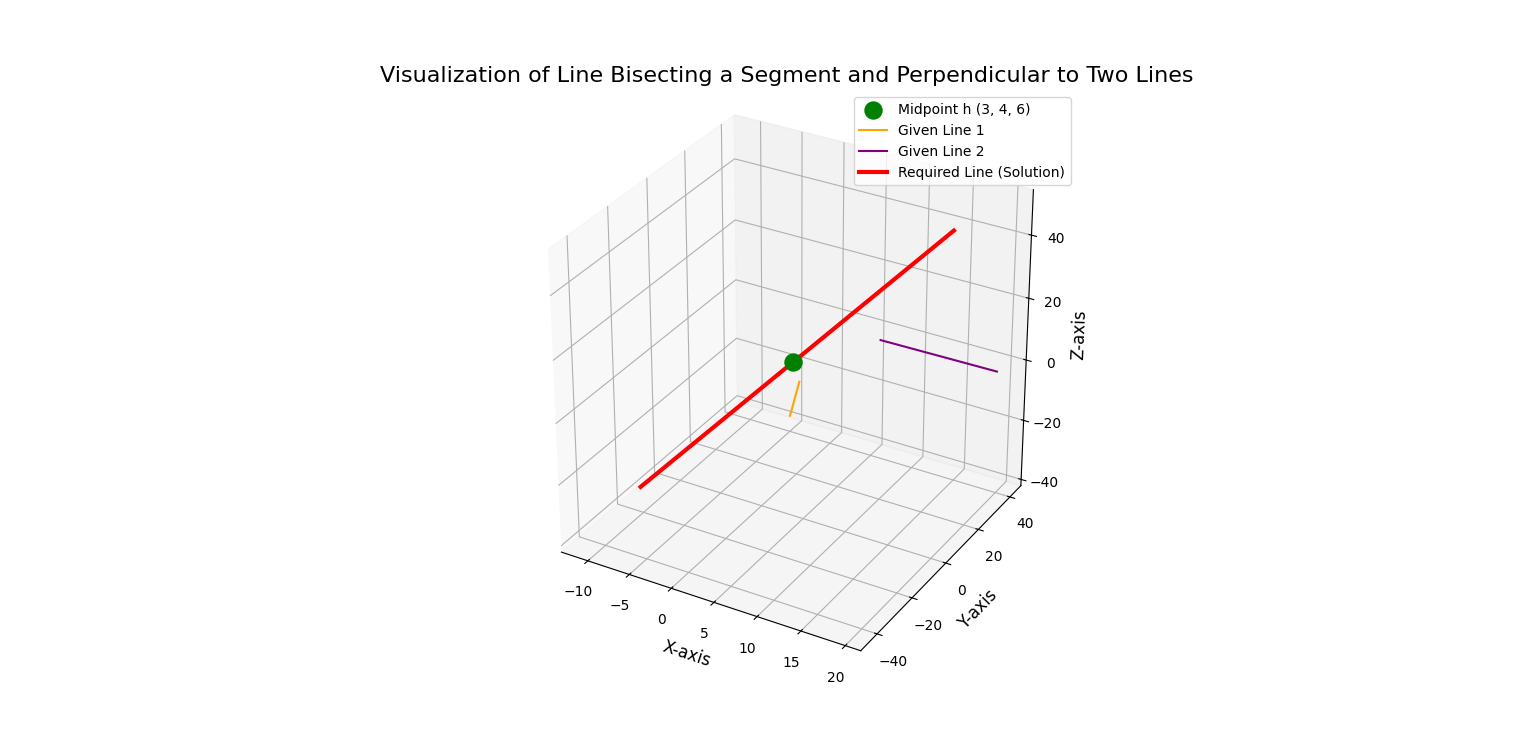
\includegraphics[width=\textwidth]{../figs/figure_py.png}
    \caption{Visualization of the solution.}
    \label{fig:final_plot}
  \end{figure}
\end{frame}

\end{document}
